\begin{flushleft}

Da zuvor noch keine Vorerfahrungen zum Erstellen von React-Apps bestand, erfolgte hier erst eine Einarbeitung in diverse Grundlagen und Funktionalitäten in  React.
React ist ein Javascript Framework zum Entwickeln von Webseiten und Webanwendungen.
Statt einfachen statischen HTML-Seiten wird hier mit sogenannten Komponenten gearbeitet, die mehrfach verwendet werden können.
Ebenso können mit States und Hooks reaktive Single-Page-Applications erstellt werden, die ein re-rendern der jeweiligen Komponenten erlauben, ohne ein Neuladen der ganzen Seite.
Weitere Pakete und Bibliotheken können mit dem Paketmanager npm ebenfalls jederzeit nachinstalliert werden.

So gibt es auch die \textit{roslibjs} Bibliothek im npm-Paketstore.
Installation und Importierung in das aktuelle Projekt wird in [\ref{frontend_install}] ausführlicher Beschrieben.
% \begin{lstlisting}[language=bash]
%     npm install roslib 
% \end{lstlisting}

% wird diese dem Projekt hinzugefügt und kann in folgender Weise inkludiert werden:

% \begin{lstlisting}
%     import ROSLIB from 'roslib';
% \end{lstlisting}

Bezüglich der Architektur, bzw. dem Aufbau der Website, haben wir uns an die standardmäßige Vorgehensweise in React gehalten, in dem man die Seite in Komponenten aufteilt und diese so an mehreren Stellen wieder verwenden kann. Dafür haben wir ein extra Verzeichnis \textit{/components} im \textit{/src} Verzeichnis angelegt, sowie eines mit \textit{/pages} für die jeweiligen Seiten. Diese werden in der \textit{App.js} Datei mit dem \textit{react-router-dom} Paket geroutet.


Wir haben uns für eine linksbündige Navigationsleiste entschieden, da diese mehr zu einem Dashboard und einer Konfigurationsseite passt. Auch hier wurde im ersten Moment nicht viel Wert auf ein besonders ausgefallenes Design gelegt. Eine schwarze Navigationsleiste mit einem aufklappbarem Burgermenü war hier für uns ausreichend. 

\hypertarget{rosboard-target}{Für} den generellen Aufbau und dem Design der Website hatten wir uns im Vorfeld schon Gedanken gemacht, so war es uns auf jeden Fall wichtig eine Übersichtseite mit allen Topics zu haben und von diesen die Inhalte auslesen zu können.
Im laufe der Wochen hatten wir ein Gespräch mit Benjamin Stähle aus dem RoboLab an der RWU, wir erzählten ihm von unserem Vorhaben und er zeigte uns ein ROS-Webdashboard namens \textit{rosboard}.
Diese Plattform hatte quasi die Funktionen, die wir für unsere Webanwendung auch geplant hatten.
Zu diesem Zeitpunkt überlegten wir uns, ob wir von nun an diese verwenden, oder unsere eigene Webanwendung programmierten.
Natürlich hätte es hier schon alle unsere gewünschten Funktionen zur Verfügung gehabt, allerdings entschieden wir uns dafür, einmal diesen Prozess von Grund auf selber zu entwickeln und unsere eigene ROS-Webanwendung zu erstellen.
Wir wollten uns aber vom Design und der Vorgehensweise trotzdem an der vorgestellten Anwendung von \textit{rosboard} orientieren.
Ebenso unterscheidet diese sich auch von der Implementierung, da diese auf ganze andere Bibliotheken basiert.
\\

\vspace{0.5cm}
Um nun die Vorteile von React in unserer Anwendung sinnvoll zu nutzen, unterteilten wir das Connection-Handling, Publishen, Subscriben oder auch beispielsweise die Auflistung der aktuellen Topics, in eigene Komponenten auf.
So konnten wir mit Hilfe von useState-Hooks und useContext-Hooks, eine Singlepage-Application bauen, die mehrere Verbindungen zu ROS-Instanzen verwalten kann.
Für jede offene Verbindung wird ein neues ROSLIB-Objekt angelegt und in ein Array gespeichert.
So kann für jedes dieser Objekte eine neue eigene Unterseite erstellt werden, um mit den ROS-Topics zu interagieren. Diese werden ebenso im Dashboard in einer Tabelle ausgegeben (siehe Abbildung \ref{fig:ros_conn}).

\begin{figure}[h!]
    \centering
    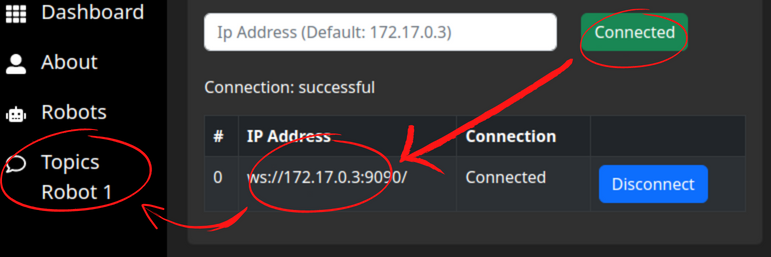
\includegraphics[width=0.8\textwidth]{imgs/web/ros_conn.png}
    \caption{Connection Handler mit Liste und automatischem Navigationspunkt}
    \label{fig:ros_conn}%
\end{figure}

Auf diesen nun generierten Topics-Unterseiten des jeweiligen Roboters, können nun Funktionen darauf angewendet werden.
Für das Publishen auf Topics haben wir uns nur auf das \textit{/cmd\_vel} Topic beschränkt, was einen recht simplem Grund hatte.
Denn zum Publishen wird natürlich auch der Message-Type der Nachricht benötigt.
Um dann dynamisch auf jedes beliebige Topic senden zu können, müsste der User ebenso, auch den entsprechenden Aufbau der Nachricht haben und diese richtig in ein Textfeld eingeben.
Dies wäre sowohl aus User Sicht sehr umständlich und fehleranfällig, da die einzelnen Werte nicht mehr in simplen vordefinierten Textfeldern, sondern in freien Textareas, hätten abgefragt werden müssen. 
Da das \textit{/cmd\_vel} Topic, welches für die Fortbewegung und Lenkung des Roboters zuständig ist, unser definitiv wichtigstes Topic war, beließen wir es dabei.
Dieser Nachrichtentyp enthält drei linear- und drei angular-Werte:
\begin{lstlisting}
    twist = {
        linear: {
            x: 0,
            y: 0,
            z: 0
        },
        angular: {
            x: 0,
            y: 0,
            z: 0
        }
    }
\end{lstlisting}
Wobei für die Fortbewegung bei Robotern, die sich auf dem Boden mit Rädern bewegen, nur die x-Werte in \textit{linear} und \textit{angular} interessant sind.
Hierfür haben wir im Frontend zwei Optionen entwickelt. 
Zum einen war es uns wichtig fest definierte Werte senden zu können, wofür wir uns für einzelne Textfelder pro Wert entschieden.
Diese wurden dann im Code auf das entsprechende Message Format (Twist) gebracht und an die \textit{rosbridge} gesendet.
Links in Abbildung \ref{fig:web_publish} sind die Textfelder, mit den jeweiligen Buttons zum Senden und Rücksetzen der Nachricht.
Bei Reset wird einfach eine neue Nachricht geschickt, die alle Werte wieder auf Null setzt.

\begin{figure}[h!]
    \centering
    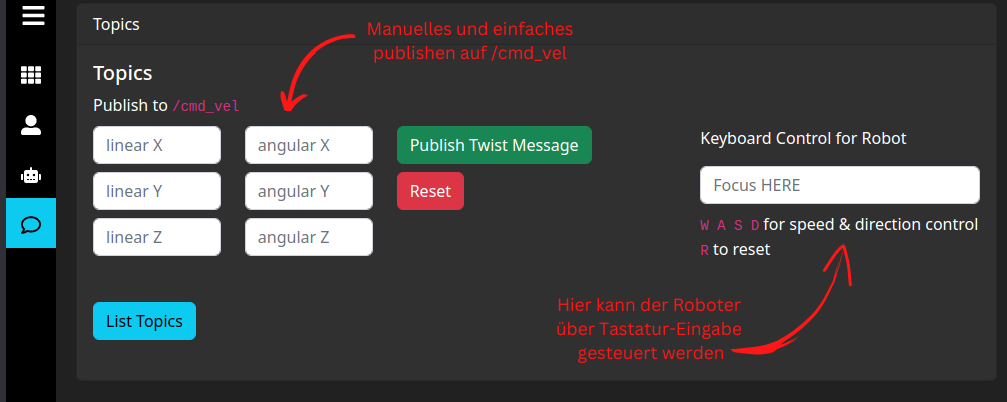
\includegraphics[width=0.8\textwidth]{imgs/web/web_publish.png}
    \caption{Zwei Möglichkeiten um auf \textit{/cmd\_vel} zu publishen}
    \label{fig:web_publish}%
\end{figure}

Ebenso dachten wir uns auch, dass es eine gute Funktionalität wäre, wenn man den Roboter über Tastatur-Eingabe steuern könnte.
So erstellten wir noch ein Textfeld, welches beim Fokussieren die Tastenfelder einließt.
Dies konnte mit dem Event-Handler \textit{onKeyPress} in React umgesetzt werden.
Durch Gedrückthalten der Tasten W, A, S, D, wird der entsprechende linear- oder angular- x-Wert inkrementiert, bzw. dekrementiert.
Mit der Taste R wird auch diese Nachricht wieder zurückgesetzt.
In Abbildung \ref{fig:web_publish} ist dies auf der rechten Seite zu sehen.
Im Anhang in [\ref{webroscomm_code}] wird einmal kurz der Vorgang des Publishen und Subscribens an einem Codebeispiel gezeigt.
\\

\vspace{0.5cm}
Als letztes soll noch auf das Subscriben zu offenen Topics über die Webanwendung beschrieben werden.
Über den Button "List Topics", werden alle momentan zur Verfügung stehenden Topics angeordnet. 
Wie in Abbildung \ref{fig:web_subscribe} zu sehen ist, öffnet sich unterhalt der Topic-Liste ein Fenster für das jeweilige Topics. 
Bei mehreren werden diese nebenbei oder darunter automatisch aufgelistet. 
Innerhalb des Festers werden alle neu ankommenden Nachrichten im JSON-Format gelistet.

\begin{figure}[h!]
    \centering
    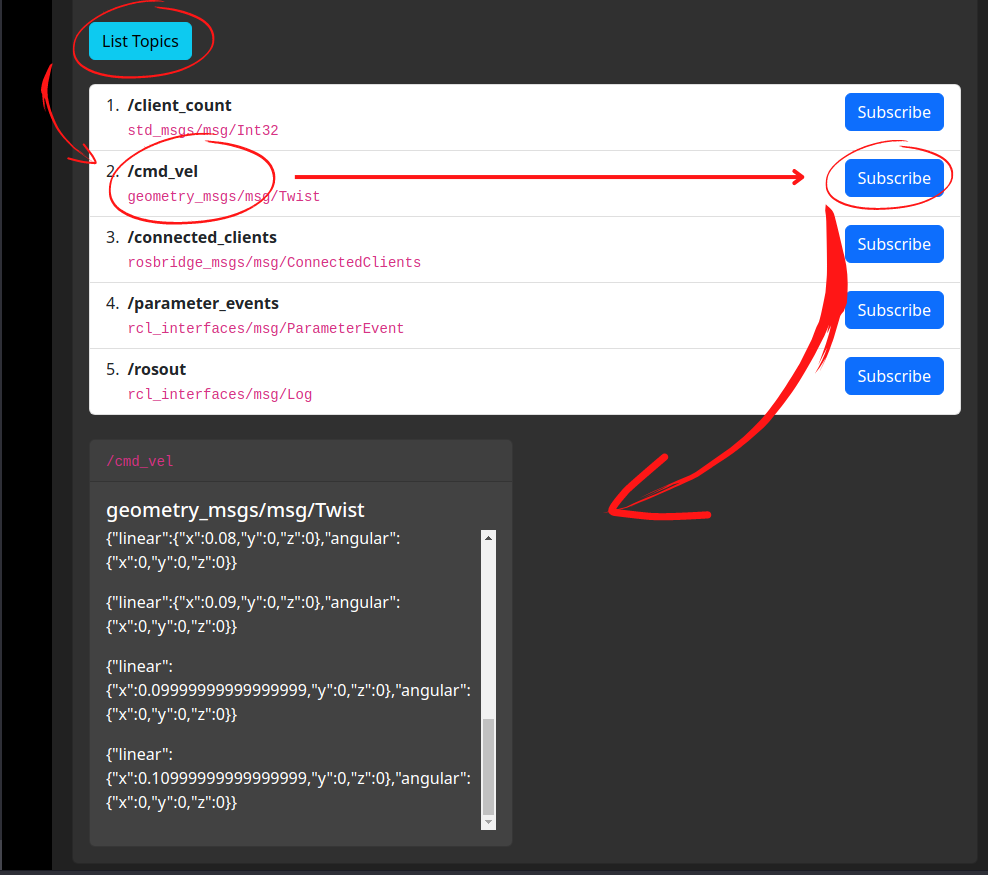
\includegraphics[width=0.8\textwidth]{imgs/web/web_subscribe.png}
    \caption{Topics Liste und Subscription zu \textit{/cmd\_vel} Topic}
    \label{fig:web_subscribe}%
\end{figure}

\end{flushleft}
    